\subsubsection{Định lượng theo size và topping}
\label{sec:inventory-demand}
Với mỗi dòng món, backend lấy định lượng size S từ Recipe. Chính sách định lượng đang dùng có hệ số S = 100\%, M = 125\%, L = 150\%; đây là cấu hình nghiệp vụ, độc lập phụ thu giá size. Thành phần có scalesWithSize=true được nhân hệ số rồi làm tròn lên theo từng ly. Thành phần có scalesWithSize=false giữ nguyên lượng. Sau đó cộng định lượng topping của một ly và nhân số ly; cuối cùng gộp tất cả dòng theo ingredientId.

Gọi $q_{ig}$ là lượng cơ bản nguyên liệu $g$ của món $i$, $r_s$ là hệ số size, $n_i$ là số ly và $t_{ig}$ là tổng lượng nguyên liệu $g$ từ topping của một ly. Khi thành phần tăng theo size:
\[
 D_g=\sum_i n_i\left(\left\lceil q_{ig}r_s\right\rceil+t_{ig}\right).
\]
Nếu không tăng theo size, thay $\lceil q_{ig}r_s\rceil$ bằng $q_{ig}$. Việc làm tròn trước khi nhân số ly bảo đảm mỗi ly đều có đủ lượng theo định mức nguyên.

\begin{table}[htbp]\centering\small
\begin{tabularx}{\linewidth}{|X|c|c|}\hline
\textbf{Thành phần} & \textbf{Một ly M} & \textbf{Hai ly M}\\\hline
Cà phê cơ bản 18g, tăng theo size & $\lceil18\times1{,}25\rceil=23$g & 46g\\\hline
Topping dùng thêm 5g cùng nguyên liệu & 5g & 10g\\\hline
Ly nhựa, không tăng theo size & 1 cái & 2 cái\\\hline
Tổng cà phê phải giữ & 28g & 56g\\\hline
\end{tabularx}\caption{Ví dụ minh họa cộng gộp định lượng, không phải công thức mặc định của topping Kem}
\end{table}

Hàm ingredientDemand dùng chung cho kiểm kho khi đặt và tính availability trên menu. Với lựa chọn một ly, số ly có thể bán bằng giá trị nhỏ nhất của $\lfloor stock_g/D_g\rfloor$ trên các nguyên liệu cần dùng. Do topping có thể dùng chung nguyên liệu với món, phải gộp demand trước khi chia; tính riêng hai phần rồi lấy min có thể báo còn hàng sai. Availability ở giao diện là ảnh chụp tham khảo; backend luôn kiểm lại tại transaction tạo đơn hoặc duyệt đổi món.

\subsubsection{Snapshot: vì sao không hoàn bằng công thức hiện tại?}
Recipe mô tả định mức bán hiện hành, trong khi snapshot là bằng chứng lượng đã giữ của một đơn cụ thể. Ví dụ khi đặt, một ly giữ 20g cà phê. Sau đó quầy sửa Recipe thành 25g. Nếu hủy bằng công thức mới, hệ thống cộng 25g dù trước đó chỉ trừ 20g, tạo ra 5g không có thật. Snapshot giữ quantity=20 nên hoàn đúng 20g. Thay topping, hệ số size hay chuyển công thức sang nguyên liệu khác cũng không thay đổi snapshot đã lưu.

Snapshot được tạo từ chính Map demand đã dùng để trừ kho, trong cùng transaction với Order. Không đọc lại Recipe sau bước trừ để dựng snapshot, vì lần đọc khác có thể không đại diện lượng vừa giữ. releasedAt là dấu hoàn; quantity vẫn giữ nguyên để tra cứu lịch sử. Một đơn có nhiều dòng món cùng dùng cà phê sẽ có một snapshot cà phê tổng, vì khi hủy toàn đơn chỉ cần trả đúng tổng lượng đã giữ.

\subsubsection{Hủy chủ động và hết thời gian giữ món}
Hủy chủ động kiểm tra chủ đơn, trạng thái và điều kiện thanh toán. Khách chỉ tự hủy PENDING/PAYMENT\_FAILED không có credit; backend khóa Order, kiểm tra các attempt cần xác minh, cập nhật trạng thái có điều kiện rồi release snapshot trong cùng transaction. Nếu bước hoàn bị lỗi thì trạng thái hủy cũng rollback. PAID và các trạng thái pha chế không dùng API hủy thông thường; đổi món đã trả tiền đi qua yêu cầu và quyết định của barista.

Với đơn bỏ thanh toán, reservationExpiresAt mặc định cách lúc tạo 30 phút. ReservationExpiryService quét khi khởi động và mỗi 30 giây, tối đa 100 đơn/lượt. Chỉ đóng đơn chưa trả tiền, chưa có bằng chứng đã thu và chưa sử dụng credit. Khi đủ điều kiện, worker hoàn snapshot và ghi CANCELLED cùng reservationExpiredAt; thông báo được phát sau commit. Giao diện hiển thị ``Đã hết thời gian đặt món, vui lòng đặt lại.'' và đưa khách về menu để tạo yêu cầu mua mới.

Deadline của đơn và deadline QR là hai giá trị khác nhau. Ví dụ đơn giữ món từ 10:00 đến 10:30; QR đầu hết 10:10 thì vẫn cấp QR mới trong thời gian còn giữ. Nếu tạo QR lúc 10:25, QR không được kéo dài quá 10:30. Backend kiểm deadline tại start payment và lúc áp dụng IPN, nên timer trình duyệt không quyết định quyền giữ kho.

Nếu tiền về muộn sau deadline, hệ thống giữ bằng chứng giao dịch, ghi REVIEW và mở hồ sơ xử lý khoản thu không áp dụng; không tự mở lại đơn, trừ kho lại hoặc gửi pha chế. Nếu worker chưa đóng đơn, callback xử lý việc đóng/hoàn trong transaction thích hợp. Các đơn đã chuyển credit hoặc có bằng chứng thu tiền được bảo toàn để quầy xử lý, tránh tự xóa giá trị khách đã trả.

\begin{figure}[p]\centering
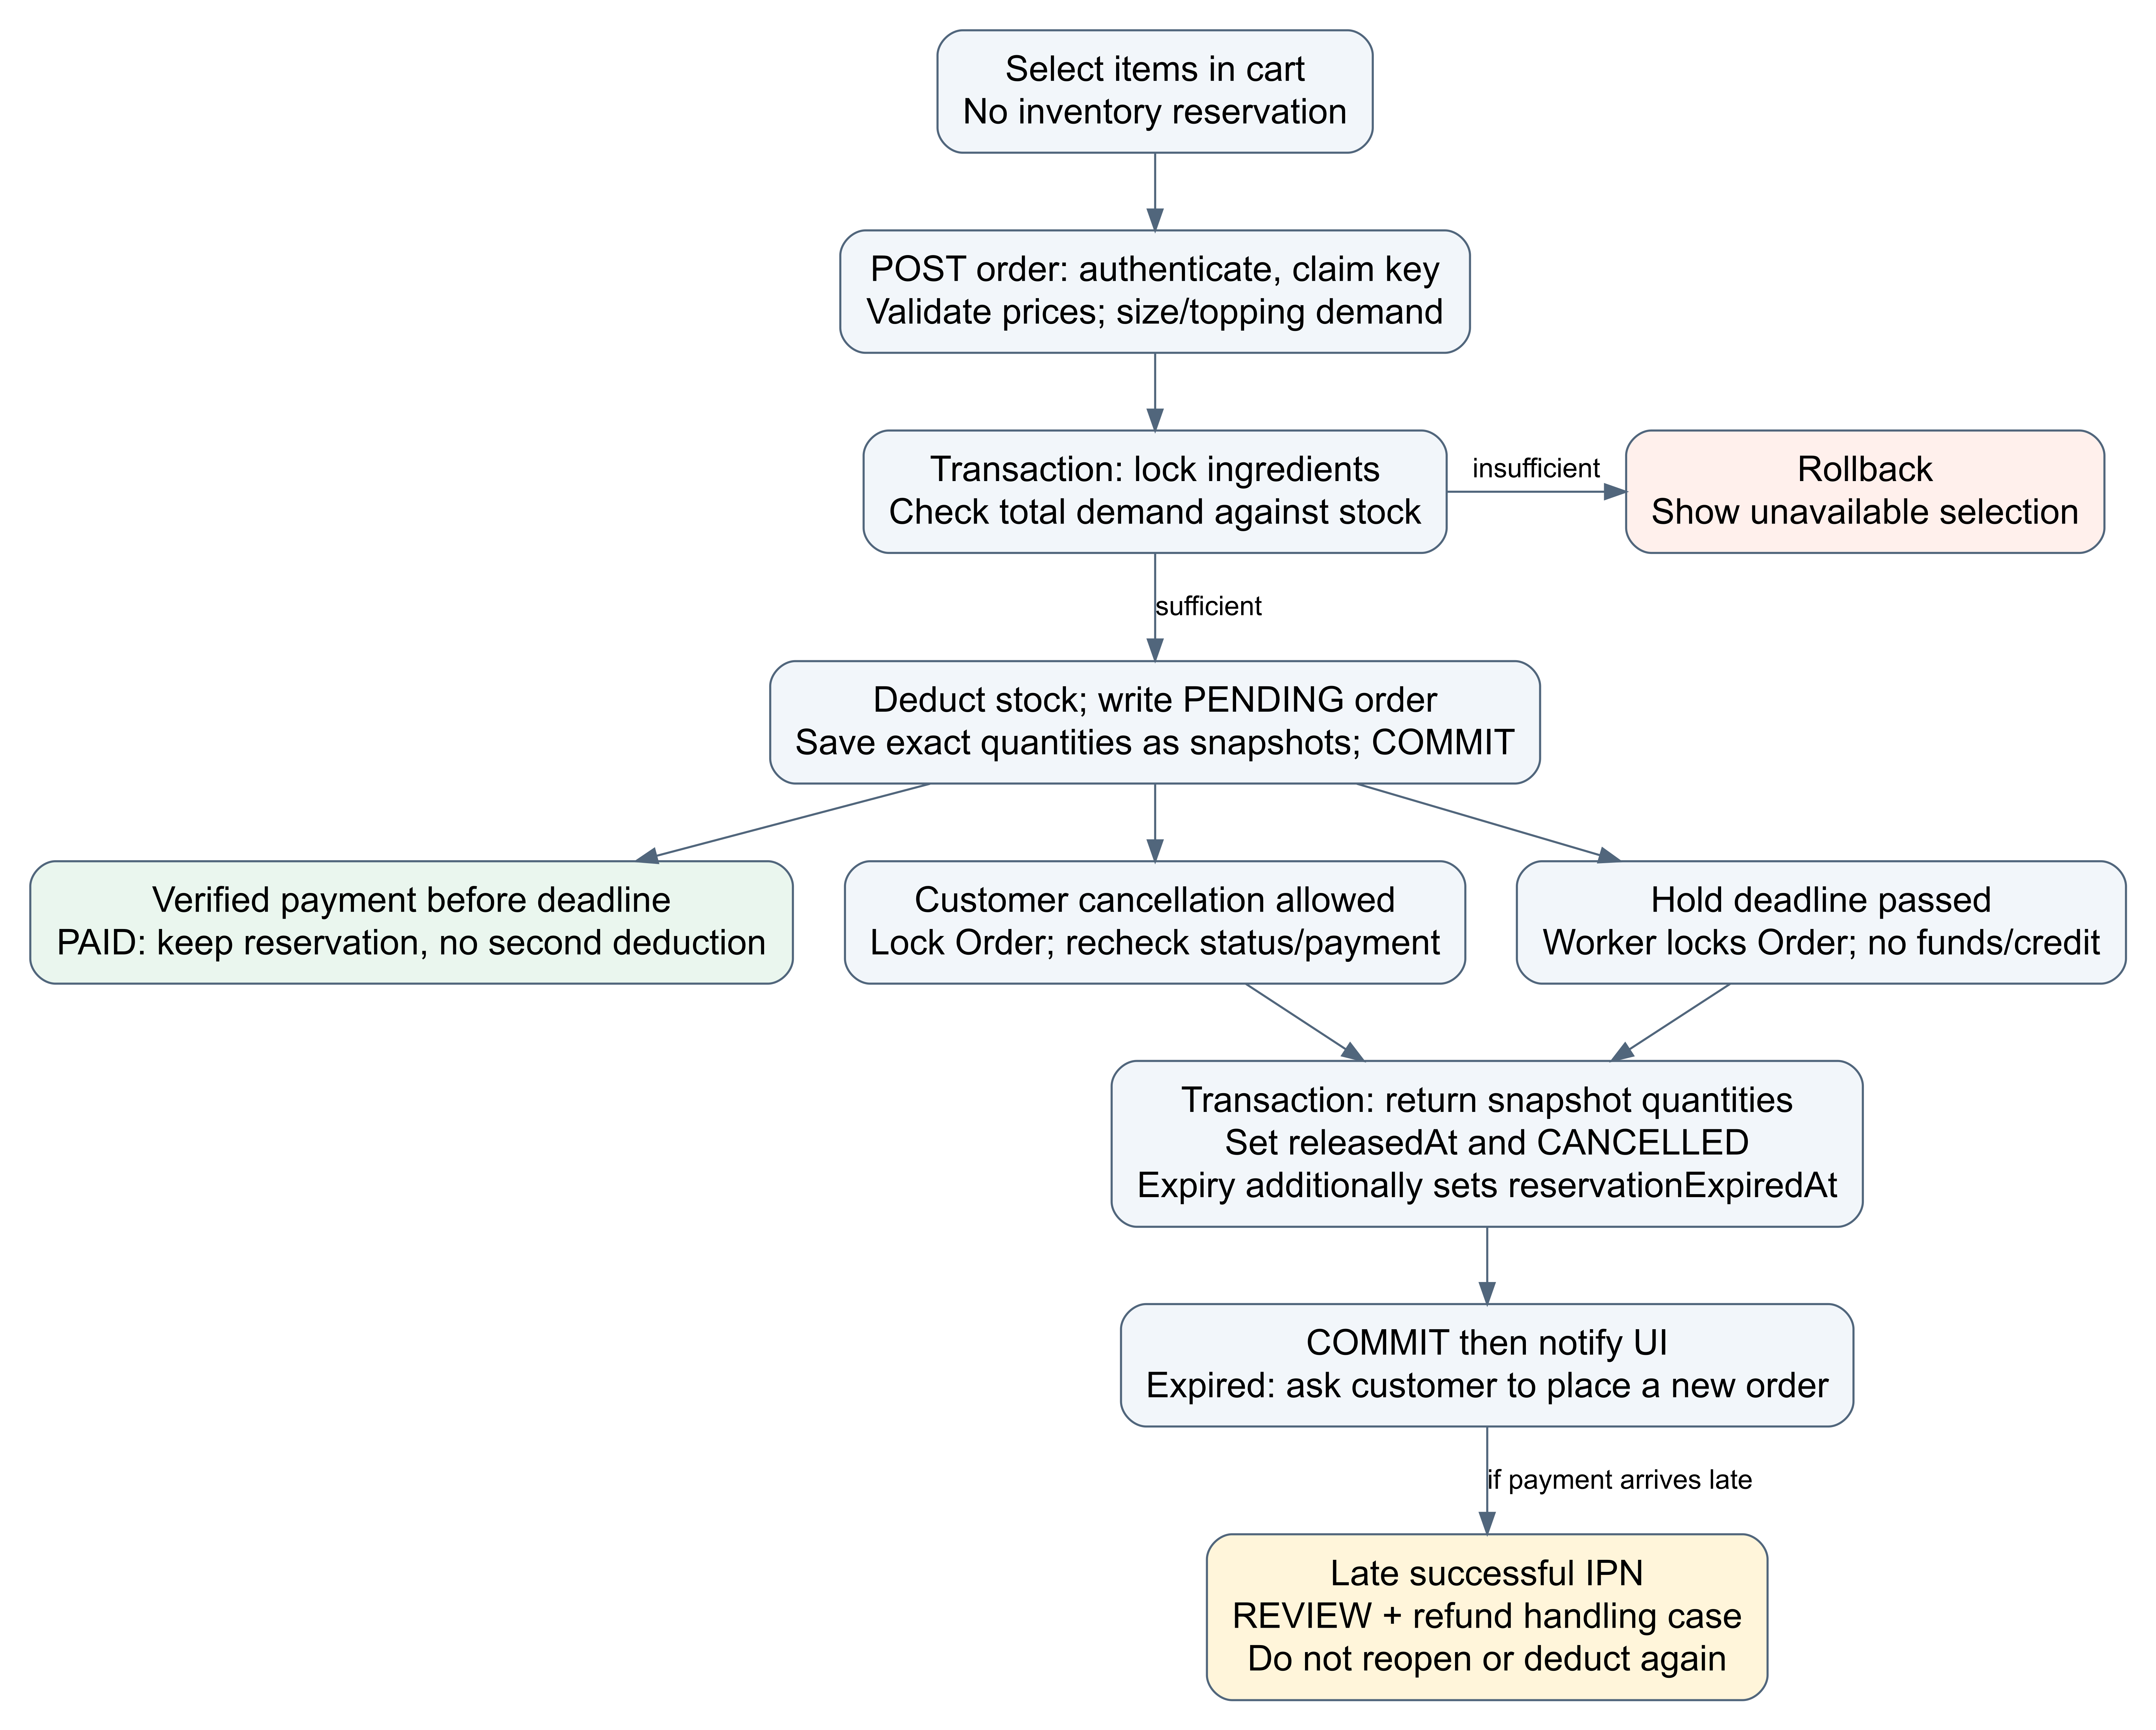
\includegraphics[width=\linewidth,height=.82\textheight,keepaspectratio]{assets/inventory/inventory-lifecycle.png}
\caption{Luồng tạo đơn, giữ kho, thanh toán, hủy và hết thời hạn giữ món}
\label{fig:inventory-lifecycle}
\end{figure}
